% Chapter Template

\chapter{Applications} % Main chapter title

\label{Applications} % Change X to a consecutive number; for referencing this chapter elsewhere, use \ref{ChapterX}

\lhead{Chapter \ref{Applications}. \emph{Applications}} % Change X to a consecutive number; this is for the header on each page - perhaps a shortened title

%----------------------------------------------------------------------------------------
%	SECTION 1
%----------------------------------------------------------------------------------------

\section{Introduction}
So far we have only covered quantised calculus on its own, 
with the aim of proving analogies of classical facts. It is natural
to wonder whether there are any uses of quantised calculus. This
chapter very briefly, and without proofs, states
some results about the application of quantised calculus to the computation
of integrals over Julia sets.

\section{The Dixmier Trace}
We have not yet discussed integration in quantised calculus. We give
a very brief overview here. The book \cite{Connes94} goes into further
detail, and the book \cite{SingularTraces} covers more technical topics.

\begin{definition}
    A linear functional $\omega \in \ell^\infty(\Ntrl)^*$ is called an extended
    limit if it satisfies the following properties:
    \begin{enumerate}
        \item{} $\|\omega\| \leq 1$.
        \item{} $\omega(a) \geq 0$ for $a \geq 0$.
        \item{} $\omega$ is shift invariant: meaning that if $S(a_0,a_1,\ldots) = (a_1,a_2,\ldots)$
        is the shift operator, then $\omega = \omega\circ S$.
    \end{enumerate}
\end{definition}    

The existence of extended limits is a consequence of the Hahn-Banach theorem,
and is proved in \cite[Thm 6.2.5]{SingularTraces}. The use
of extended limits is in the definition of a Dixmier trace.
The following isproved in \cite[Ch. 2]{SingularTraces}.
\begin{proposition}
    Let $\omega$ be an extended limit, and let $T > 0$ be an operator
    in $\M_{1,\infty}$. Define,
    \begin{equation}
        \Tr_\omega(T) := \omega\left\{\frac{1}{\log(N+1)}\sum_{k=0}^N \mu_k(T)\right\}_{N > 0}.
    \end{equation}
    Then $\Tr_\omega$ is additive, and extends to a linear functional
    on all of $\M_{1,\infty}$. $\Tr_\omega$ is called a Dixmier trace.
\end{proposition}

\section{Julia Sets}
\begin{definition}
    Let $c \in \Cplx$, and let $\varphi_c(z) = z^2+c$. Define
    \begin{equation}
        B := \{z \in \Cplx\;:\; \|\{\varphi^n(z)\}_{n \geq 0}\|_\infty < \infty\}.
    \end{equation}
    Let $J$, the Julia set associated to $\varphi_c$, be the boundary of $B$,
    $J:= \partial B$.
    
    When $c$ is small, it can be shown that $J$ is a Jordan curve
    whose complement has two connected components, an interior and exterior.
\end{definition}
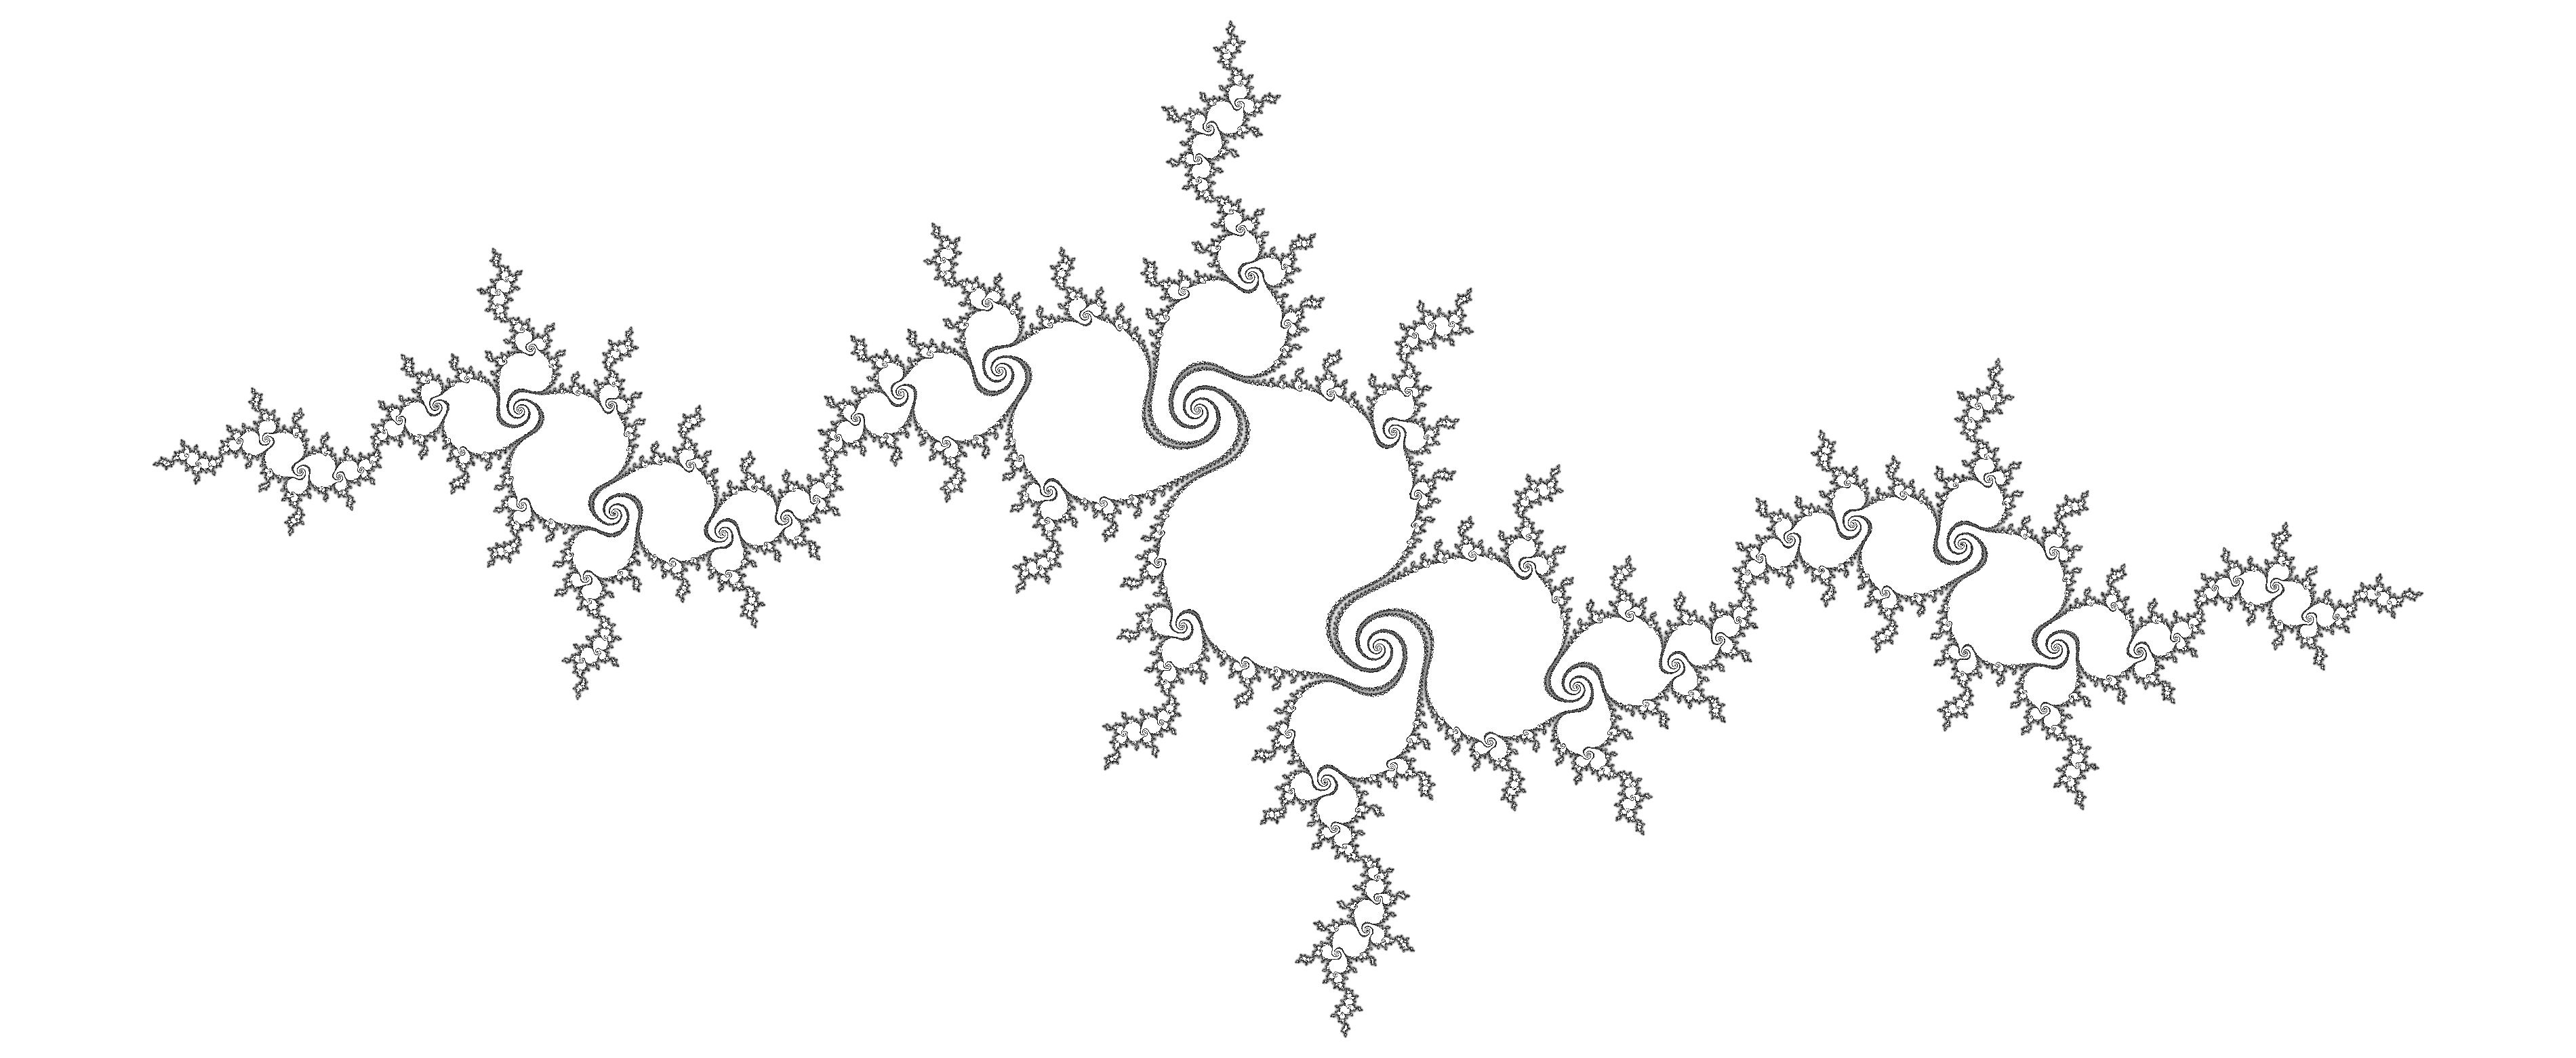
\includegraphics[width=160mm]{Pictures/Julia_set.png}\\
The above shows $J$ for $c = -1.12+0.222i$.
The conformal mapping theorem states that there is a holomorphic
bijection $Z$ between the open unit disc $\{z \in \Cplx\;:\;|z| < 1\}$
and the interior of $B$. There is a result of Caratheodory
which states that $Z$ extends to a continuous
map from $\Circ$ to $J$. 

The Hausdorff dimension of $J$, $p$, is known to be in $(0,1)$. Let
$f:J\to\Cplx$. We consider the quantity
\begin{equation}
    \Tr_\omega(f(Z)|\qd Z|^p).
\end{equation}
It is argued by Connes in \cite{Connes94} that in fact this is a sensible
means of integrating functions on $J$. Herein lies the utility
of quantised calculus.
